Peers on the Catalyst network can assume a variety of roles. These include:

\begin{itemize}

\item \textbf{User node} - The default state of all nodes on the network. The role of a user node is to receive transactions, check the  validity of transactions and when valid, forward these to their peers. User nodes can also generate transactions and observe the network. However, they are not entitled nor required to perform any other work on the network. 

\item \textbf{Reservist node} - A node that has signalled its intent to perform work for the network and provided proofs of its available computing resource dedicated to the network.

\item \textbf{Worker node} - A node that has been granted a worker pass for a finite period of time. 

\item \textbf{Producer node} - A worker node that has been selected to perform work for a particular ledger cycle. A producer node will be rewarded for performing good quality work by receiving KAT tokens. 

\item \textbf{Storage node} - A node able to sell some of its spare storage to allow other users to store their data in a decentralised manner. 

\end{itemize}

All nodes on the network will receive transactions, validate and forward these transactions to other peers that they are connected to. This is to allow efficient propagation of transactions across the network. \\

\begin{figure}
\centering
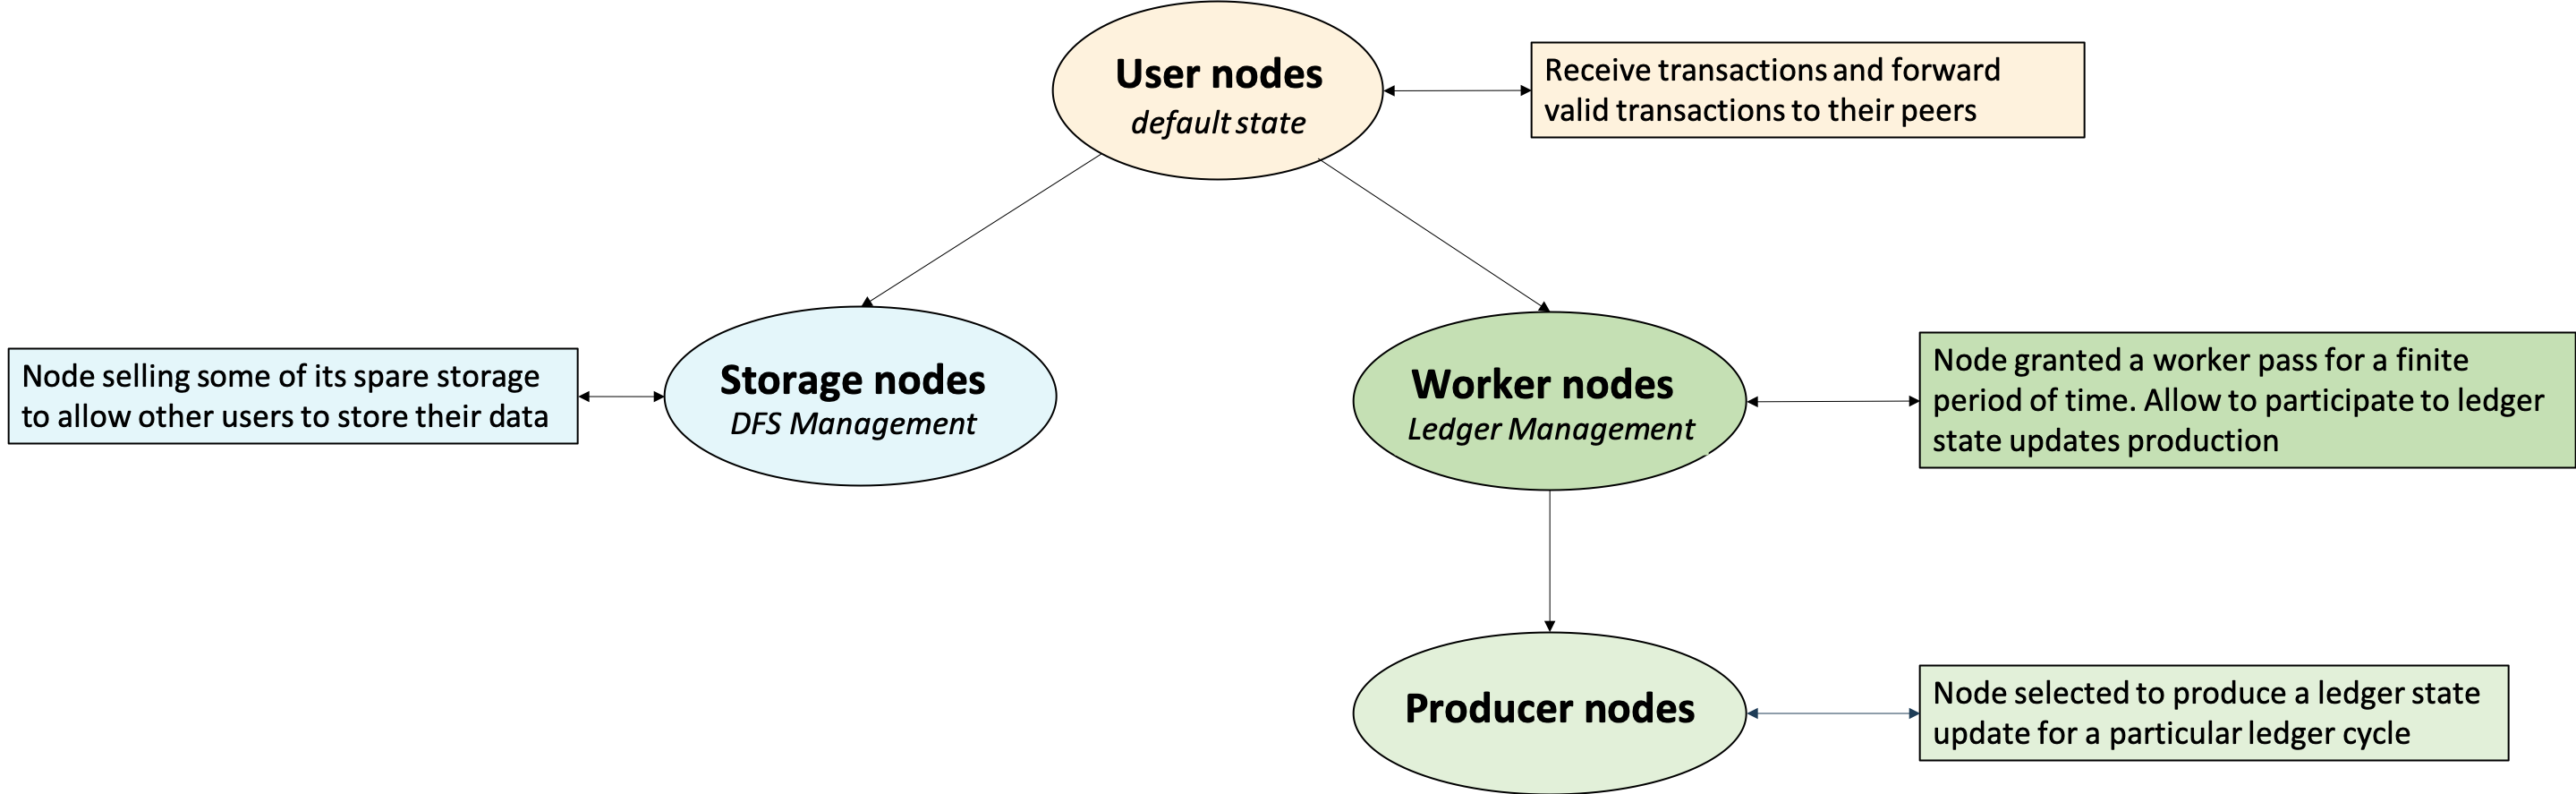
\includegraphics[width=12cm]{Figures/Node_roles}
\caption{\label{fig:nr}Illustration of the different roles assumed by nodes on Catalyst Network.}
\end{figure}


Reservist nodes, upon registering to perform work on the network, are placed at the back of a node queue (or worker queue) from which they must wait to be given a worker pass. This pass grants them the right to become a worker node and a member of the worker pool for a finite period of time. During this period of time, several ledger cycles happen and the worker node has a chance of being randomly selected to become a producer node for any ledger cycle. The producer nodes are the network peers that work together and follow a consensus-based protocol to build the ledger state updates, as described in section~\ref{Sec:Dem}. 